Much of the teaching in this book is geared towards enabling you to
write fast code, whether this is through the choice of the right
method, or through optimal coding of a method. Consequently, you
sometimes want to measure just \emph{how fast} your code is. If you
have a simulation that runs for many hours, you'd think just looking
on the clock would be enough measurement. However, as you wonder
whether your code could be faster than it is, you need more detailed
measurements. This tutorial will teach you some ways to measure the
behaviour of your code in more or less detail.

Here we will discuss 
\begin{itemize}
\item timers: ways of measuring the execution time (and sometimes
  other measurements) of a particular piece of code, and
\item profiling tools: ways of measuring how much time each piece of
  code, typically a subroutine, takes during a specific run.
\end{itemize}

\Level 0 {Timers}

There are various ways of timing your code, but mostly they come down
to calling a routine twice that tells you the clock values:
\begin{verbatim}
  tstart = clockticks()
  ....
  tend = clockticks()
  runtime = (tend-tstart)/ticks_per_sec
\end{verbatim}
For instance, in Fortran there is the \n{system_clock}
routine\index{systemclock@\n{system_clock}}:
\verbatiminput{code/papi/timers/ftimer.F}
with output
\begin{verbatim}
 Clock frequency:       10000
   1.000000       813802544   813826097   2.000000  
\end{verbatim}
In C there is the \n{clock} function:
\verbatiminput{code/papi/timers/ctimer.c}
with output
\begin{verbatim}
clock resolution: 1000000
res: 1.000000e+00
start/stop: 0.000000e+00,2.310000e+00
Time: 2.310000e+00
\end{verbatim}
Do you see a difference between the Fortran and C approaches? Hint:
what happens in both cases when the execution time becomes long? At
what point do you run into trouble?

\Level 1 {System utilities}

There are unix system calls that can be used for timing: \n{getrusage}
and \n{gettimeofday}. These timers have the advantage that they can
distinguish between user time and system time, that is, exclusively
timing program execution or giving \indexterm{wallclock time}
including all system activities.

\Level 0 {Accurate counters}

The timers in the previous section had a resolution of at best a
millisecond, which corresponds to several thousand cycles on a modern
CPU. For more accurate counting it is typically necessary to use
assembly language, such as the Intel \n{RDTSC} (ReaD Time Stamp
Counter)
instruction~\url{http://developer.intel.com/drg/pentiumII/appnotes/RDTSCPM1.HTM}. However,
this approach of using processor-specific timers is not portable. For
this reason, the PAPI package (\url{http://icl.cs.utk.edu/papi/})
provides a uniform interface to timers and other performance
counters. You can see this package in action in the codes in
appendix~\ref{app:codes}.

\Level 0 {Profiling tools}

Profiling tools will give you the time spent in various events in the
program, typically functions and subroutines, or parts of the code
that you have declared as such. The tool will then report how many
time the event occurred, total and average time spent, et cetera.

The only tool we mention here is \indexterm{gprof}, the profiler of
the \indexterm{GNU} compiler. There are other tools, such as
\indexterm{TAU}, which have great sophistication, but go beyond this
tutorial. Finally, we mention that the \indexterm{PETSc} library
allows you to define your own timers and events.

\begin{verbatim}
% gcc  -g -pg ./srcFile.
% gprof    ./exeFile gmon.out > profile.txt
% gprof -l ./exeFile gmon.out > profile_line.txt
% gprof -A ./exeFile gmon.out > profile_anotated.tx
\end{verbatim}

\Level 1 {MPI profiling}

The MPI library has been designed to make it easy to profile. Each
function such as \n{MPI_Send} does no more than calling
\n{PMPI_Send}. This means that a profiling library can redefine
\n{MPI_Send} to
\begin{itemize}
\item initialize a profiling stage,\item call \n{PMPI_Send}, \item
  finish the profiling stage.
\end{itemize}

\Level 0 {Tracing}

In profiling we are only concerned with aggregate information: how
many times a routine was called, and with what total/average/min/max
runtime. However sometimes we want to know about the exact timing of
events. This is especially relevant in a parallel context when we care
about \indextermbus{load}{unbalance} and \indexterm{idle time}.

Tools such as Vampyr can collect trace information about
events and in particular messages, and render them in displays such as
figure~\ref{fig:vampyr}.
\begin{figure}[ht]
  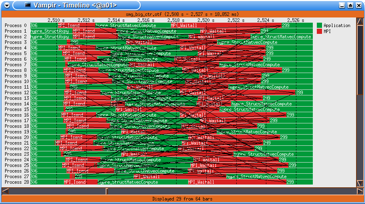
\includegraphics{graphics-public/vampyrtrace}
  \caption{A Vampyr timeline diagram of a parallel process.}
  \label{fig:vampyr}
\end{figure}
